\documentclass{standalone}
\usepackage{tikz}
\usetikzlibrary{patterns, positioning}


\begin{document}
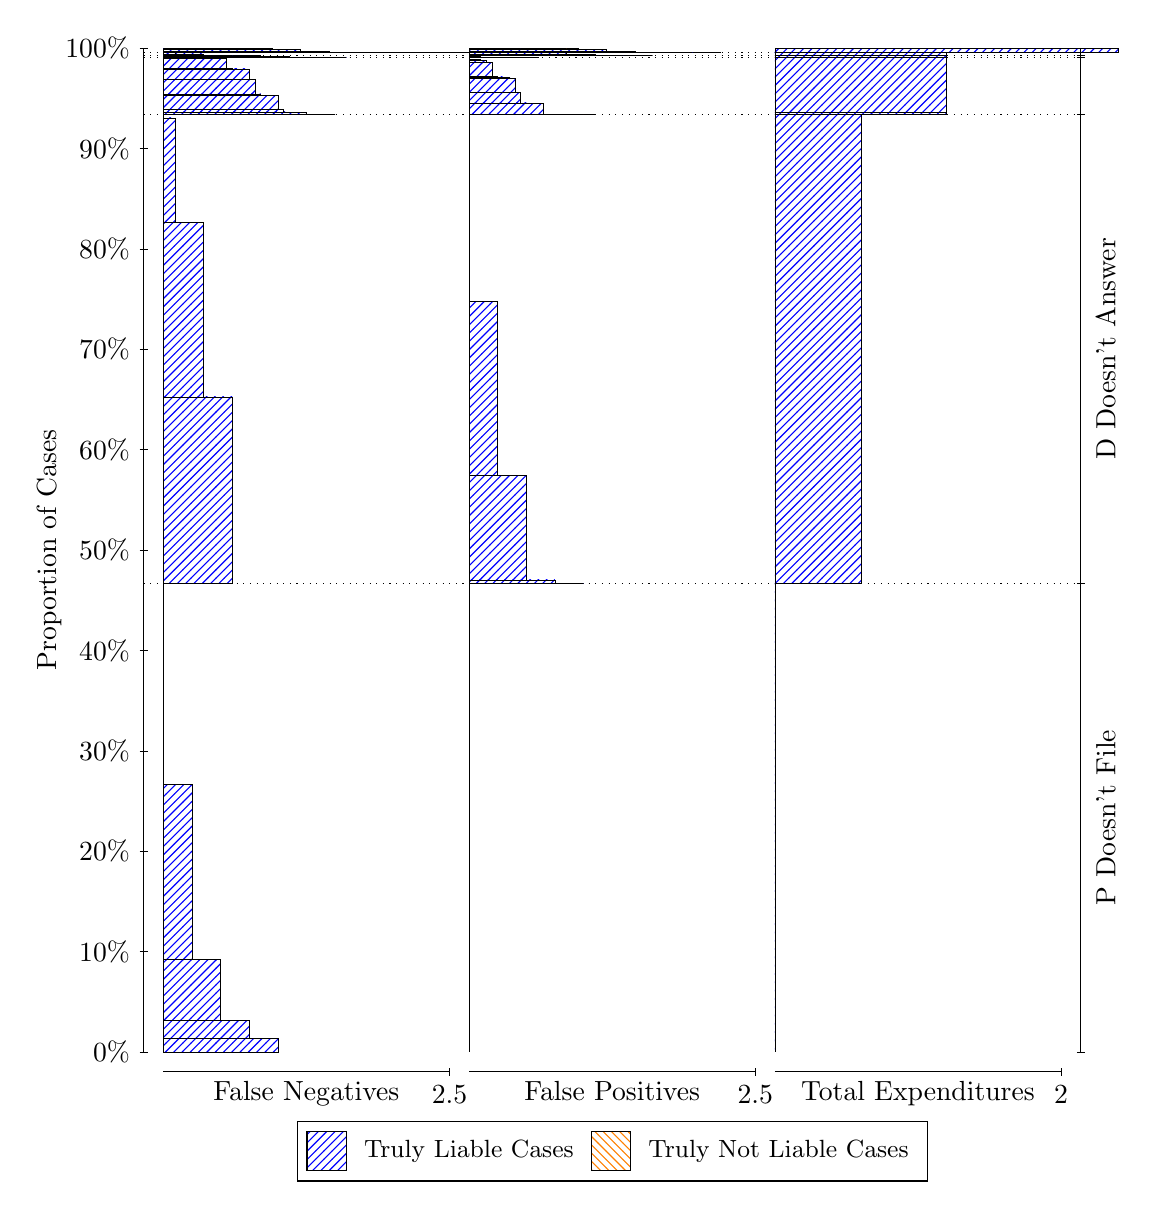
\begin{tikzpicture}
\draw[black, very thin] (1.5,1.75) -- (1.5,14.5);
\node[rotate=90, text=black, anchor=center] at (0.3, 8.125) {Proportion of Cases};
\draw[black, very thin] (1.45,1.75) -- (1.55,1.75);
\node[text=black, anchor=east] at (1.45, 1.75) {0\%};
\draw[black, very thin] (1.45,3.025) -- (1.55,3.025);
\node[text=black, anchor=east] at (1.45, 3.025) {10\%};
\draw[black, very thin] (1.45,4.3) -- (1.55,4.3);
\node[text=black, anchor=east] at (1.45, 4.3) {20\%};
\draw[black, very thin] (1.45,5.575) -- (1.55,5.575);
\node[text=black, anchor=east] at (1.45, 5.575) {30\%};
\draw[black, very thin] (1.45,6.85) -- (1.55,6.85);
\node[text=black, anchor=east] at (1.45, 6.85) {40\%};
\draw[black, very thin] (1.45,8.125) -- (1.55,8.125);
\node[text=black, anchor=east] at (1.45, 8.125) {50\%};
\draw[black, very thin] (1.45,9.4) -- (1.55,9.4);
\node[text=black, anchor=east] at (1.45, 9.4) {60\%};
\draw[black, very thin] (1.45,10.675) -- (1.55,10.675);
\node[text=black, anchor=east] at (1.45, 10.675) {70\%};
\draw[black, very thin] (1.45,11.95) -- (1.55,11.95);
\node[text=black, anchor=east] at (1.45, 11.95) {80\%};
\draw[black, very thin] (1.45,13.225) -- (1.55,13.225);
\node[text=black, anchor=east] at (1.45, 13.225) {90\%};
\draw[black, very thin] (1.45,14.5) -- (1.55,14.5);
\node[text=black, anchor=east] at (1.45, 14.5) {100\%};

\draw[black, very thin] (13.4,1.75) -- (13.4,14.5);
\draw[black, very thin] (13.35,1.75) -- (13.45,1.75);
\node[anchor=west] at (13.35, 1.75) {};
\draw[black, very thin] (13.35,7.6993) -- (13.45,7.6993);
\node[anchor=west] at (13.35, 7.6993) {};
\draw[black, very thin] (13.35,13.658) -- (13.45,13.658);
\node[anchor=west] at (13.35, 13.658) {};
\draw[black, very thin] (13.35,14.379) -- (13.45,14.379);
\node[anchor=west] at (13.35, 14.379) {};
\draw[black, very thin] (13.35,14.402) -- (13.45,14.402);
\node[anchor=west] at (13.35, 14.402) {};
\draw[black, very thin] (13.35,14.444) -- (13.45,14.444);
\node[anchor=west] at (13.35, 14.444) {};
\draw[black, very thin] (13.35,14.5) -- (13.45,14.5);
\node[anchor=west] at (13.35, 14.5) {};

\draw[black, very thin, pattern color=blue, pattern=north east lines] (1.75,1.75) rectangle (3.2033,1.9205);
\draw[black, very thin, pattern color=blue, pattern=north east lines] (1.75,1.9205) rectangle (2.84,2.1473);
\draw[black, very thin, pattern color=blue, pattern=north east lines] (1.75,2.1473) rectangle (2.4767,2.9271);
\draw[black, very thin, pattern color=blue, pattern=north east lines] (1.75,2.9271) rectangle (2.1133,5.1525);
\draw[black, very thin, pattern color=orange, pattern=north west lines] (1.75,5.1525) rectangle (1.75,5.1525);
\draw[black, very thin, pattern color=blue, pattern=north east lines] (1.75,5.1525) rectangle (1.75,7.6993);
\draw[black, very thin, pattern color=blue, pattern=north east lines] (1.75,7.6993) rectangle (2.622,10.07);
\draw[black, very thin, pattern color=blue, pattern=north east lines] (1.75,10.07) rectangle (2.2587,12.288);
\draw[black, very thin, pattern color=blue, pattern=north east lines] (1.75,12.288) rectangle (1.8953,13.612);
\draw[black, very thin, pattern color=orange, pattern=north west lines] (1.75,13.612) rectangle (1.75,13.612);
\draw[black, very thin, pattern color=blue, pattern=north east lines] (1.75,13.612) rectangle (1.75,13.658);
\draw[black, very thin, pattern color=blue, pattern=north east lines] (1.75,13.658) rectangle (3.93,13.658);
\draw[black, very thin, pattern color=blue, pattern=north east lines] (1.75,13.658) rectangle (3.7847,13.658);
\draw[black, very thin, pattern color=blue, pattern=north east lines] (1.75,13.658) rectangle (3.6393,13.659);
\draw[black, very thin, pattern color=blue, pattern=north east lines] (1.75,13.659) rectangle (3.5667,13.681);
\draw[black, very thin, pattern color=blue, pattern=north east lines] (1.75,13.681) rectangle (3.494,13.681);
\draw[black, very thin, pattern color=blue, pattern=north east lines] (1.75,13.681) rectangle (3.4213,13.683);
\draw[black, very thin, pattern color=blue, pattern=north east lines] (1.75,13.683) rectangle (3.3487,13.69);
\draw[black, very thin, pattern color=blue, pattern=north east lines] (1.75,13.69) rectangle (3.276,13.718);
\draw[black, very thin, pattern color=blue, pattern=north east lines] (1.75,13.718) rectangle (3.2033,13.902);
\draw[black, very thin, pattern color=blue, pattern=north east lines] (1.75,13.902) rectangle (3.1307,13.903);
\draw[black, very thin, pattern color=blue, pattern=north east lines] (1.75,13.903) rectangle (3.058,13.905);
\draw[black, very thin, pattern color=blue, pattern=north east lines] (1.75,13.905) rectangle (2.9853,13.917);
\draw[black, very thin, pattern color=blue, pattern=north east lines] (1.75,13.917) rectangle (2.9127,14.103);
\draw[black, very thin, pattern color=blue, pattern=north east lines] (1.75,14.103) rectangle (2.84,14.236);
\draw[black, very thin, pattern color=blue, pattern=north east lines] (1.75,14.236) rectangle (2.7673,14.236);
\draw[black, very thin, pattern color=blue, pattern=north east lines] (1.75,14.236) rectangle (2.6947,14.236);
\draw[black, very thin, pattern color=blue, pattern=north east lines] (1.75,14.236) rectangle (2.622,14.238);
\draw[black, very thin, pattern color=blue, pattern=north east lines] (1.75,14.238) rectangle (2.5493,14.376);
\draw[black, very thin, pattern color=blue, pattern=north east lines] (1.75,14.376) rectangle (2.4767,14.378);
\draw[black, very thin, pattern color=blue, pattern=north east lines] (1.75,14.378) rectangle (2.404,14.378);
\draw[black, very thin, pattern color=blue, pattern=north east lines] (1.75,14.378) rectangle (2.3313,14.378);
\draw[black, very thin, pattern color=blue, pattern=north east lines] (1.75,14.378) rectangle (2.2587,14.378);
\draw[black, very thin, pattern color=blue, pattern=north east lines] (1.75,14.378) rectangle (2.186,14.379);
\draw[black, very thin, pattern color=blue, pattern=north east lines] (1.75,14.379) rectangle (2.0407,14.379);
\draw[black, very thin, pattern color=blue, pattern=north east lines] (1.75,14.379) rectangle (1.8953,14.379);
\draw[black, very thin, pattern color=orange, pattern=north west lines] (1.75,14.379) rectangle (1.75,14.379);
\draw[black, very thin, pattern color=blue, pattern=north east lines] (1.75,14.379) rectangle (4.0753,14.379);
\draw[black, very thin, pattern color=blue, pattern=north east lines] (1.75,14.379) rectangle (3.712,14.384);
\draw[black, very thin, pattern color=blue, pattern=north east lines] (1.75,14.384) rectangle (3.3487,14.396);
\draw[black, very thin, pattern color=blue, pattern=north east lines] (1.75,14.396) rectangle (2.9853,14.402);
\draw[black, very thin, pattern color=blue, pattern=north east lines] (1.75,14.402) rectangle (2.622,14.402);
\draw[black, very thin, pattern color=orange, pattern=north west lines] (1.75,14.402) rectangle (1.75,14.402);
\draw[black, very thin, pattern color=blue, pattern=north east lines] (1.75,14.402) rectangle (2.622,14.402);
\draw[black, very thin, pattern color=blue, pattern=north east lines] (1.75,14.402) rectangle (2.2587,14.425);
\draw[black, very thin, pattern color=blue, pattern=north east lines] (1.75,14.425) rectangle (1.8953,14.444);
\draw[black, very thin, pattern color=orange, pattern=north west lines] (1.75,14.444) rectangle (1.75,14.444);
\draw[black, very thin, pattern color=blue, pattern=north east lines] (1.75,14.444) rectangle (1.75,14.444);
\draw[black, very thin, pattern color=blue, pattern=north east lines] (1.75,14.444) rectangle (5.8193,14.444);
\draw[black, very thin, pattern color=blue, pattern=north east lines] (1.75,14.444) rectangle (5.456,14.444);
\draw[black, very thin, pattern color=blue, pattern=north east lines] (1.75,14.444) rectangle (5.0927,14.445);
\draw[black, very thin, pattern color=blue, pattern=north east lines] (1.75,14.445) rectangle (4.7293,14.448);
\draw[black, very thin, pattern color=blue, pattern=north east lines] (1.75,14.448) rectangle (4.584,14.448);
\draw[black, very thin, pattern color=blue, pattern=north east lines] (1.75,14.448) rectangle (4.366,14.448);
\draw[black, very thin, pattern color=blue, pattern=north east lines] (1.75,14.448) rectangle (4.2207,14.448);
\draw[black, very thin, pattern color=blue, pattern=north east lines] (1.75,14.448) rectangle (4.0027,14.448);
\draw[black, very thin, pattern color=blue, pattern=north east lines] (1.75,14.448) rectangle (3.8573,14.458);
\draw[black, very thin, pattern color=blue, pattern=north east lines] (1.75,14.458) rectangle (3.494,14.486);
\draw[black, very thin, pattern color=blue, pattern=north east lines] (1.75,14.486) rectangle (3.1307,14.499);
\draw[black, very thin, pattern color=blue, pattern=north east lines] (1.75,14.499) rectangle (2.7673,14.5);
\draw[black, very thin, pattern color=blue, pattern=north east lines] (1.75,14.5) rectangle (2.404,14.5);
\draw[black, very thin, pattern color=blue, pattern=north east lines] (1.75,14.5) rectangle (2.0407,14.5);
\draw[black, very thin, pattern color=orange, pattern=north west lines] (1.75,14.5) rectangle (1.75,14.5);
\draw[black, very thin, pattern color=orange, pattern=north west lines] (5.6333,1.75) rectangle (5.6333,1.75);
\draw[black, very thin, pattern color=blue, pattern=north east lines] (5.6333,1.75) rectangle (5.6333,7.6993);
\draw[black, very thin, pattern color=orange, pattern=north west lines] (5.6333,7.6993) rectangle (7.0867,7.6993);
\draw[black, very thin, pattern color=blue, pattern=north east lines] (5.6333,7.6993) rectangle (7.0867,7.6993);
\draw[black, very thin, pattern color=blue, pattern=north east lines] (5.6333,7.6993) rectangle (6.7233,7.7452);
\draw[black, very thin, pattern color=blue, pattern=north east lines] (5.6333,7.7452) rectangle (6.36,9.0691);
\draw[black, very thin, pattern color=blue, pattern=north east lines] (5.6333,9.0691) rectangle (5.9967,11.287);
\draw[black, very thin, pattern color=blue, pattern=north east lines] (5.6333,11.287) rectangle (5.6333,13.658);
\draw[black, very thin, pattern color=orange, pattern=north west lines] (5.6333,13.658) rectangle (7.232,13.658);
\draw[black, very thin, pattern color=blue, pattern=north east lines] (5.6333,13.658) rectangle (7.232,13.658);
\draw[black, very thin, pattern color=orange, pattern=north west lines] (5.6333,13.658) rectangle (7.0867,13.658);
\draw[black, very thin, pattern color=blue, pattern=north east lines] (5.6333,13.658) rectangle (7.0867,13.658);
\draw[black, very thin, pattern color=orange, pattern=north west lines] (5.6333,13.658) rectangle (6.9413,13.658);
\draw[black, very thin, pattern color=blue, pattern=north east lines] (5.6333,13.658) rectangle (6.9413,13.659);
\draw[black, very thin, pattern color=blue, pattern=north east lines] (5.6333,13.659) rectangle (6.8687,13.659);
\draw[black, very thin, pattern color=orange, pattern=north west lines] (5.6333,13.659) rectangle (6.796,13.659);
\draw[black, very thin, pattern color=blue, pattern=north east lines] (5.6333,13.659) rectangle (6.796,13.659);
\draw[black, very thin, pattern color=blue, pattern=north east lines] (5.6333,13.659) rectangle (6.7233,13.659);
\draw[black, very thin, pattern color=orange, pattern=north west lines] (5.6333,13.659) rectangle (6.6507,13.659);
\draw[black, very thin, pattern color=blue, pattern=north east lines] (5.6333,13.659) rectangle (6.6507,13.661);
\draw[black, very thin, pattern color=blue, pattern=north east lines] (5.6333,13.661) rectangle (6.578,13.799);
\draw[black, very thin, pattern color=blue, pattern=north east lines] (5.6333,13.799) rectangle (6.5053,13.801);
\draw[black, very thin, pattern color=blue, pattern=north east lines] (5.6333,13.801) rectangle (6.4327,13.801);
\draw[black, very thin, pattern color=blue, pattern=north east lines] (5.6333,13.801) rectangle (6.36,13.802);
\draw[black, very thin, pattern color=blue, pattern=north east lines] (5.6333,13.802) rectangle (6.2873,13.934);
\draw[black, very thin, pattern color=blue, pattern=north east lines] (5.6333,13.934) rectangle (6.2147,14.12);
\draw[black, very thin, pattern color=blue, pattern=north east lines] (5.6333,14.12) rectangle (6.142,14.132);
\draw[black, very thin, pattern color=blue, pattern=north east lines] (5.6333,14.132) rectangle (6.0693,14.134);
\draw[black, very thin, pattern color=blue, pattern=north east lines] (5.6333,14.134) rectangle (5.9967,14.135);
\draw[black, very thin, pattern color=blue, pattern=north east lines] (5.6333,14.135) rectangle (5.924,14.319);
\draw[black, very thin, pattern color=blue, pattern=north east lines] (5.6333,14.319) rectangle (5.8513,14.347);
\draw[black, very thin, pattern color=blue, pattern=north east lines] (5.6333,14.347) rectangle (5.7787,14.354);
\draw[black, very thin, pattern color=blue, pattern=north east lines] (5.6333,14.354) rectangle (5.706,14.356);
\draw[black, very thin, pattern color=blue, pattern=north east lines] (5.6333,14.356) rectangle (5.6333,14.379);
\draw[black, very thin, pattern color=orange, pattern=north west lines] (5.6333,14.379) rectangle (6.5053,14.379);
\draw[black, very thin, pattern color=blue, pattern=north east lines] (5.6333,14.379) rectangle (6.5053,14.38);
\draw[black, very thin, pattern color=blue, pattern=north east lines] (5.6333,14.38) rectangle (6.142,14.386);
\draw[black, very thin, pattern color=blue, pattern=north east lines] (5.6333,14.386) rectangle (5.7787,14.397);
\draw[black, very thin, pattern color=blue, pattern=north east lines] (5.6333,14.397) rectangle (5.6333,14.402);
\draw[black, very thin, pattern color=orange, pattern=north west lines] (5.6333,14.402) rectangle (7.9587,14.402);
\draw[black, very thin, pattern color=blue, pattern=north east lines] (5.6333,14.402) rectangle (7.9587,14.402);
\draw[black, very thin, pattern color=blue, pattern=north east lines] (5.6333,14.402) rectangle (7.5953,14.402);
\draw[black, very thin, pattern color=blue, pattern=north east lines] (5.6333,14.402) rectangle (7.232,14.421);
\draw[black, very thin, pattern color=blue, pattern=north east lines] (5.6333,14.421) rectangle (6.8687,14.444);
\draw[black, very thin, pattern color=blue, pattern=north east lines] (5.6333,14.444) rectangle (6.5053,14.444);
\draw[black, very thin, pattern color=orange, pattern=north west lines] (5.6333,14.444) rectangle (8.8307,14.444);
\draw[black, very thin, pattern color=blue, pattern=north east lines] (5.6333,14.444) rectangle (8.8307,14.444);
\draw[black, very thin, pattern color=blue, pattern=north east lines] (5.6333,14.444) rectangle (8.4673,14.444);
\draw[black, very thin, pattern color=orange, pattern=north west lines] (5.6333,14.444) rectangle (8.4673,14.444);
\draw[black, very thin, pattern color=blue, pattern=north east lines] (5.6333,14.444) rectangle (8.4673,14.444);
\draw[black, very thin, pattern color=blue, pattern=north east lines] (5.6333,14.444) rectangle (8.104,14.445);
\draw[black, very thin, pattern color=orange, pattern=north west lines] (5.6333,14.445) rectangle (8.104,14.445);
\draw[black, very thin, pattern color=blue, pattern=north east lines] (5.6333,14.445) rectangle (8.104,14.445);
\draw[black, very thin, pattern color=blue, pattern=north east lines] (5.6333,14.445) rectangle (7.7407,14.448);
\draw[black, very thin, pattern color=orange, pattern=north west lines] (5.6333,14.448) rectangle (7.7407,14.448);
\draw[black, very thin, pattern color=blue, pattern=north east lines] (5.6333,14.448) rectangle (7.7407,14.458);
\draw[black, very thin, pattern color=blue, pattern=north east lines] (5.6333,14.458) rectangle (7.3773,14.458);
\draw[black, very thin, pattern color=blue, pattern=north east lines] (5.6333,14.458) rectangle (7.3773,14.486);
\draw[black, very thin, pattern color=blue, pattern=north east lines] (5.6333,14.486) rectangle (7.014,14.496);
\draw[black, very thin, pattern color=orange, pattern=north west lines] (5.6333,14.496) rectangle (6.8687,14.496);
\draw[black, very thin, pattern color=blue, pattern=north east lines] (5.6333,14.496) rectangle (6.8687,14.496);
\draw[black, very thin, pattern color=blue, pattern=north east lines] (5.6333,14.496) rectangle (6.6507,14.496);
\draw[black, very thin, pattern color=orange, pattern=north west lines] (5.6333,14.496) rectangle (6.5053,14.496);
\draw[black, very thin, pattern color=blue, pattern=north east lines] (5.6333,14.496) rectangle (6.5053,14.496);
\draw[black, very thin, pattern color=blue, pattern=north east lines] (5.6333,14.496) rectangle (6.2873,14.496);
\draw[black, very thin, pattern color=blue, pattern=north east lines] (5.6333,14.496) rectangle (6.142,14.499);
\draw[black, very thin, pattern color=blue, pattern=north east lines] (5.6333,14.499) rectangle (5.7787,14.5);
\draw[black, very thin, pattern color=blue, pattern=north east lines] (5.6333,14.5) rectangle (5.6333,14.5);
\draw[black, very thin, pattern color=orange, pattern=north west lines] (9.5167,1.75) rectangle (9.5167,1.75);
\draw[black, very thin, pattern color=blue, pattern=north east lines] (9.5167,1.75) rectangle (9.5167,7.6993);
\draw[black, very thin, pattern color=orange, pattern=north west lines] (9.5167,7.6993) rectangle (10.607,7.6993);
\draw[black, very thin, pattern color=blue, pattern=north east lines] (9.5167,7.6993) rectangle (10.607,13.658);
\draw[black, very thin, pattern color=orange, pattern=north west lines] (9.5167,13.658) rectangle (11.697,13.658);
\draw[black, very thin, pattern color=blue, pattern=north east lines] (9.5167,13.658) rectangle (11.697,13.678);
\draw[black, very thin, pattern color=orange, pattern=north west lines] (9.5167,13.678) rectangle (11.697,13.678);
\draw[black, very thin, pattern color=blue, pattern=north east lines] (9.5167,13.678) rectangle (11.697,14.379);
\draw[black, very thin, pattern color=orange, pattern=north west lines] (9.5167,14.379) rectangle (11.697,14.379);
\draw[black, very thin, pattern color=blue, pattern=north east lines] (9.5167,14.379) rectangle (11.697,14.402);
\draw[black, very thin, pattern color=orange, pattern=north west lines] (9.5167,14.402) rectangle (11.697,14.402);
\draw[black, very thin, pattern color=blue, pattern=north east lines] (9.5167,14.402) rectangle (11.697,14.444);
\draw[black, very thin, pattern color=orange, pattern=north west lines] (9.5167,14.444) rectangle (13.877,14.444);
\draw[black, very thin, pattern color=blue, pattern=north east lines] (9.5167,14.444) rectangle (13.877,14.448);
\draw[black, very thin, pattern color=orange, pattern=north west lines] (9.5167,14.448) rectangle (13.877,14.448);
\draw[black, very thin, pattern color=blue, pattern=north east lines] (9.5167,14.448) rectangle (13.877,14.5);
\draw[black, dotted] (1.5,7.6993) -- (13.4,7.6993);
\draw[black, dotted] (1.5,13.658) -- (13.4,13.658);
\draw[black, dotted] (1.5,14.379) -- (13.4,14.379);
\draw[black, dotted] (1.5,14.402) -- (13.4,14.402);
\draw[black, dotted] (1.5,14.444) -- (13.4,14.444);
\draw[black, very thin] (1.75,1.5) -- (5.3833,1.5);
\node[text=black, anchor=north] at (3.5667, 1.5) {False Negatives};
\draw[black, very thin] (5.3833,1.45) -- (5.3833,1.55);
\node[text=black, anchor=north] at (5.3833, 1.45) {2.5};

\draw[black, very thin] (5.6333,1.5) -- (9.2667,1.5);
\node[text=black, anchor=north] at (7.45, 1.5) {False Positives};
\draw[black, very thin] (9.2667,1.45) -- (9.2667,1.55);
\node[text=black, anchor=north] at (9.2667, 1.45) {2.5};

\draw[black, very thin] (9.5167,1.5) -- (13.15,1.5);
\node[text=black, anchor=north] at (11.333, 1.5) {Total Expenditures};
\draw[black, very thin] (13.15,1.45) -- (13.15,1.55);
\node[text=black, anchor=north] at (13.15, 1.45) {2};

\node[text=black, centered, rotate=90] at (13.72, 4.7246) {P Doesn't File};
\node[text=black, centered, rotate=90] at (13.72, 10.678) {D Doesn't Answer};





\draw (7.449999999999999,1.5) node[draw=none] (baseCoordinate) {};
\begin{scope}[align=center]
        \matrix[scale=0.5, draw=black, below=0.5cm of baseCoordinate, nodes={draw}, column sep=0.1cm]{
            \node[rectangle, draw, minimum width=0.5cm, minimum height=0.5cm, pattern color=blue, pattern=north east lines] {}; &
            \node[draw=none, font=\small, text=black] (B) {Truly Liable Cases}; &
            \node[rectangle, draw, minimum width=0.5cm, minimum height=0.5cm, pattern color=orange, pattern=north west lines] {}; &
            \node[draw=none, font=\small, text=black] (B) {Truly Not Liable Cases}; \\
            };
\end{scope}

\end{tikzpicture}
\end{document}